% !TeX program = xelatex
% PDF para pdfpc: cada página = lámina (izquierda) + notas del orador (derecha).
% Uso: pdfpc -n right -w both -d 15 presentacion_con_notas.pdf
% Requiere compilar antes presentacion_avance.pdf
\documentclass{article}
\usepackage[paperwidth=320mm,paperheight=90mm,margin=0pt]{geometry}
\usepackage{fontspec}
\setmainfont{Inter}[BoldFont={Inter SemiBold},ItalicFont={Inter Italic},BoldItalicFont={Inter SemiBold Italic}]
\usepackage[spanish,es-noshorthands]{babel}
\usepackage{graphicx}
\usepackage{xcolor}
\usepackage{enumitem}
\usepackage{tikz}
\definecolor{ink}{HTML}{1F2933}
\definecolor{muted}{HTML}{66727F}
\definecolor{accent}{HTML}{0E6F7C}
\definecolor{warm}{HTML}{C2511A}
\pagestyle{empty}
\setlength{\parindent}{0pt}
\setlist[itemize]{leftmargin=5mm,itemsep=1.6mm,topsep=0pt,label=\textcolor{accent}{\textbullet}}

% Frase para decir tal cual
\newcommand{\di}[1]{\textcolor{accent}{“#1”}}

% \nota{página}{título}{tiempo}{acumulado}{ítems}
\newcommand{\nota}[5]{%
  \null
  \begin{tikzpicture}[remember picture,overlay]
    \node[anchor=north west,inner sep=0pt] at (current page.north west)
      {\includegraphics[width=160mm,height=90mm,page=#1]{presentacion_avance.pdf}};
    \node[anchor=north west,inner sep=0pt,text width=146mm,align=left,font=\fontsize{12}{14}\selectfont]
      at ([xshift=167mm,yshift=-6mm]current page.north west)
      {\textbf{#1 · #2}\hfill\textcolor{muted}{#3\quad|\quad llevo #4}};
    \draw[muted!40,line width=0.6pt] ([xshift=167mm,yshift=-12mm]current page.north west) -- ++(146mm,0);
    \node[anchor=north west,inner sep=0pt,text width=146mm,align=left,font=\fontsize{13.5}{17}\selectfont,text=ink]
      at ([xshift=167mm,yshift=-15.5mm]current page.north west)
      {\begin{itemize}#5\end{itemize}};
  \end{tikzpicture}
  \newpage}

\begin{document}

\nota{1}{Portada}{20 s}{0:20}{%
  \item Frase de inicio, de memoria: \di{En quince minutos van a saber por qué un paquete LoRa llega o se pierde, y cómo decidir si un simulador que calcula eso en milisegundos dice la verdad.}
  \item Sin “buenas tardes, hoy les voy a presentar”.
  \item Reloj: vuelta completa = 5 min de FLoRa; astilla roja = 8 ms de FAST-LoRa.}

\nota{2}{Problema}{60 s}{1:20}{%
  \item 100 sensores; 6 SF × 8 potencias = 48 opciones cada uno → $10^{168}$ redes.
  \item Preguntar \di{¿Cuánto creen que se demora evaluar una?} y aguantar 5 a 7 s en silencio.
  \item FLoRa: más de 5 min. FAST-LoRa: menos de 8 ms (200 nodos).
  \item Decir: diez mil evaluaciones son más de un mes contra poco más de un minuto.
  \item Pasar con \di{Eso es lo que vende el paper. Pero hay un problema.}}

\nota{3}{Sin embargo}{70 s}{2:30}{%
  \item PDR = fracción de paquetes que llegan.
  \item Leer la caja naranja como una sola frase.
  \item ADR = ajuste automático de SF y potencia: justo lo que la herramienta promete evaluar.
  \item \di{Los números que no calzan los van a ver en el estado del arte.}
  \item Cerrar mirando al público con la frase de abajo.}

\nota{4}{Promesa}{25 s}{2:55}{%
  \item Decirla explícita: \di{Al terminar van a saber cuándo creerle a un simulador de 8 ms.}
  \item Nombrar los 3 bloques. Arriba a la derecha se ve en cuál vamos.}

\nota{5}{LoRaWAN}{60 s}{3:55}{%
  \item Ejemplo primero: el sensor de riego de la franja de abajo.
  \item \di{Miren el 1}: transmite sin escuchar el canal. ALOHA puro, lo del curso, máx. 18\,\%.
  \item \di{El 2}: el mismo paquete llega a dos gateways; basta uno.
  \item \di{El 3}: el servidor descarta duplicados y ajusta SF y potencia: eso es el ADR.
  \item Pasar con \di{¿Y qué es el SF que tanto se repite?}}

\nota{6}{Spreading factor}{50 s}{4:45}{%
  \item Cada SF extra hace el símbolo dos veces más largo.
  \item Con 10 bytes (los del código), de SF7 a SF12: 27 veces más tiempo en el aire.
  \item Más tiempo en el aire = más energía y más choques.
  \item Sorpresa: SF12 entiende una señal 100 veces más débil que el ruido ($-20$ dB).}

\nota{7}{Llega débil}{45 s}{5:30}{%
  \item Primera razón para perder un paquete.
  \item La potencia baja con la distancia y además varía al azar: por eso es una campana.
  \item A la derecha de la línea llega: esa área es $\psi$. A la izquierda se pierde.}

\nota{8}{Choca}{60 s}{6:30}{%
  \item Segunda razón.
  \item B pisa los últimos 5 símbolos del preámbulo y A no es 6 dB más fuerte → A se pierde.
  \item Con SF distintos casi siempre sobrevive.
  \item No chocar = $\zeta$. PDR = $\psi\cdot\zeta$; con varios gateways basta que uno reciba.}

\nota{9}{Simular vs calcular}{45 s}{7:15}{%
  \item IDEA CENTRAL, tal cual: \di{FLoRa cuenta paquetes, FAST-LoRa calcula probabilidades.}
  \item FLoRa: 5 días simulados, unos 432 paquetes por nodo.
  \item FAST-LoRa: $\psi$ y $\zeta$ para todos los nodos de una vez.
  \item Cerco: sin bajada, un canal, tráfico estable.
  \item Control de tiempo: aquí deberían ir unos 7:15.}

\nota{10}{Mapa}{60 s}{8:15}{%
  \item Izquierda: ALOHA y geometría estocástica (red promedio).
  \item Medio: modelos por dispositivo (Toro-Betancur, FAST-LoRa).
  \item Derecha: LoRaSim, ns-3, FLoRa; al extremo, una red física.
  \item La flecha es lo que voy a comparar.
  \item Pie: 4 citas, 3 del mismo grupo, ninguna réplica.}

\nota{11}{Lecturas}{55 s}{9:10}{%
  \item Contar solo tres tarjetas.
  \item Bor: de ahí salen los parámetros de propagación (medidos en Lancaster).
  \item Croce: los SF se interfieren un poco → umbrales.
  \item Toro-Betancur ya tenía este modelo en 2021; FAST-LoRa lo toma vía Zhang 2023.
  \item Si hay tiempo, Lima: en otro entorno cambian los parámetros.}

\nota{12}{Cabos sueltos}{70 s}{10:20}{%
  \item \di{Leí el paper con calculadora en mano y encontré cuatro cosas.}
  \item 1: el tamaño del paquete no está; en el código: 10 bytes.
  \item 2: 0,040 promedia por nodo; 0,038 es el promedio simple de la tabla.
  \item 3: 15 s contra 0,6 ms → unas $10^4$ veces, no $10^3$.
  \item 4: ec. 11 usa $2\sigma$; corresponde $\sqrt2\sigma$ (respaldo 21).}

\nota{13}{Código}{65 s}{11:25}{%
  \item \di{Como faltaba el payload, fui al código.}
  \item Experimentos en otro repositorio del autor, con su FLoRa modificado.
  \item Tiempo en el aire distinto (FLoRa: 20 B fijos y símbolos extra).
  \item Umbral mismo SF: 6 contra 1 dB. Matriz al revés. El ADR falla.
  \item Con $\lambda = 0{,}001$ algunas pesan poco: medirlo es el aporte.}

\nota{14}{Objetivo}{50 s}{12:15}{%
  \item Leer el diagrama de izquierda a derecha.
  \item Criterio de éxito fijado ANTES de simular.
  \item Si no calza, explicar por qué también es un resultado.
  \item Entregables: figuras propias, tablas de error, repositorio público.
  \item Control: si van más de 13:15, saltar el plan.}

\nota{15}{Resultado}{50 s}{13:05}{%
  \item \di{En la final van a ver esta figura y esta tabla, hechas por mí.}
  \item 1: un nodo y un gateway (144 corridas).
  \item 2: redes densas (80 corridas); el naranjo, 1,044, es el peor caso.
  \item 3: los tiempos salen de las mismas corridas.}

\nota{16}{Plan · saltable}{25 s}{13:30}{%
  \item Tres fases: instalar FLoRa 1.1.0 + Exp. 1 → Exp. 2 y 3 → comparar, informe, repositorio.
  \item Riesgo: versión antigua (OMNeT++ 6.0, INET 4.4); si falla, escribir a los autores.}

\nota{17}{Referencias}{10 s}{13:40}{%
  \item Solo unos segundos: \di{Cada afirmación lleva su número de referencia.}}

\nota{18}{Cierre}{40 s}{14:20}{%
  \item Idea central por tercera vez: milisegundos contra minutos; hay que verificarlo por fuera.
  \item \di{Creerle lo suficiente para usarlo, dudar lo suficiente para verificarlo.}
  \item Nombrar los 4 aportes.
  \item Cerrar: \di{Quedo atento a sus comentarios, sobre todo si alguien ha usado FLoRa.}
  \item Dejar esta lámina durante las preguntas (no avanzar).}

\nota{19}{Respaldo: parámetros}{preguntas}{--}{%
  \item Todo sale de las Tablas 1 a 3 del paper.
  \item El payload (10 B) solo aparece en el código.
  \item Para volver al cierre: tecla g, escribir 18, Enter.}

\nota{20}{Respaldo: código}{preguntas}{--}{%
  \item Repos: jaznrp/FastLoRa (el citado redirige ahí) y jaznrp/MultiAgent-MARLTC.
  \item Con $\lambda = 0{,}001$ el traslape entre dos nodos es menor a 0,2\,\%.
  \item El código recibe el payload en bits; FLoRa ignora el valor configurado.}

\nota{21}{Respaldo: ecuación 11}{preguntas}{--}{%
  \item Resta de dos gaussianas independientes: varianza $2\sigma^2$, desviación $\sqrt2\sigma$.
  \item El paper y el código usan $2\sigma$ (varianza $4\sigma^2$).
  \item Pesa más con nodos del mismo SF que llegan con potencias parecidas.}

\nota{22}{Respaldo: Packet Tracer}{preguntas}{--}{%
  \item Packet Tracer y GNS3 emulan redes IP; no modelan la capa física LoRa.
  \item FLoRa y ns-3 sí; FLoRa es la referencia del paper.}

\nota{23}{Respaldo: tiempo en el aire}{preguntas}{--}{%
  \item Depende mucho del payload: casi el doble entre 20 y 51 bytes.
  \item Por eso importa que el paper no informe $L$.}

\end{document}
